\documentclass[aspectratio=169]{beamer}
\usepackage{will_handley_beamer}
\usepackage{title_page}

% Commands
% --------
% - \arxiv{arxiv number}
% - \arxiv{<number>}            arxiv.org/abs/<number>
% - \oldarxiv{<arxiv number>}   arxiv.org/<number>
% - \doi{<doi>}                 doi.org/<doi>
% - \xkcd{<number>}             xkcd.com/<number>
% - \email{<email>}             <<email>>
% - \tthref{<website>}          <website>
% - \av[dist]{<quantity>}       <quantity>_{dist}
% - \student{<name>}{<detail>}{<photo>}

% Talk details
% ------------
\title{\texttt{lsbi}: linear simulation based inference }
\date{11\textsuperscript{th} September 2024}

\begin{document}

\begin{frame}
    \titlepage
\end{frame}

\begin{frame}
    \frametitle{Context from phystat}
    \begin{itemize}
        \item From \textbf{Jesse Thaler}'s talk on Interpretable Machine Learning:
            \begin{quote}
                ``If asked what is the most under-used Machine Learning technique in physics\ldots\\ \hfill\ldots my answer is only half jokingly \textbf{linear regression}.''
            \end{quote}
        \item sbi mentioned in (so far)
            \begin{itemize}
                \item Monday
                    \begin{itemize}
                        \item Ben Wandelt: Cosmology and machine learning¶
                        \item Maximilian Dax: Simulation-based machine learning for gravitational-wave analysis
                        \item Andre Scaffidi: Anomaly aware machine learning for dark matter direct detection at the DARWIN experiment
                        \item Joshua Villarrea: Feldman-Cousins’ ML Cousin
                    \end{itemize}
            \end{itemize}
    \end{itemize}
\end{frame}

\begin{frame}
    \frametitle{Who?}
    \begin{columns}
        \column{0.8\textwidth}
    Idea I've been working on/talking about for the better part of 18 months,
    \begin{itemize}
        \item Nicolas Mediato Diaz (MSci project)
        \item David Yallup (Postdoc)
        \item Thomas Gessey Jones (Postdoc)
    \end{itemize}

    Many others have also presented this idea independently
    \begin{itemize}
        \item \texttt{SELFI} incorporates much of this idea: Leclercq~\arxiv{1902.10149}
        \item some of these ideas are in \texttt{MOPED}: Heavens~\oldarxiv{astro-ph/9911102}
        \item Also appears in Häggström~\arxiv{2403.07454}
    \end{itemize}
        
        \column{0.2\textwidth}
        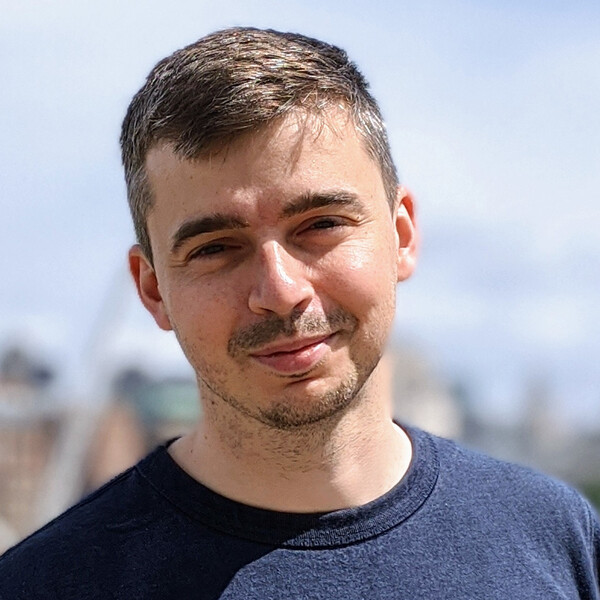
\includegraphics[width=\textwidth]{people/david_yallup}
        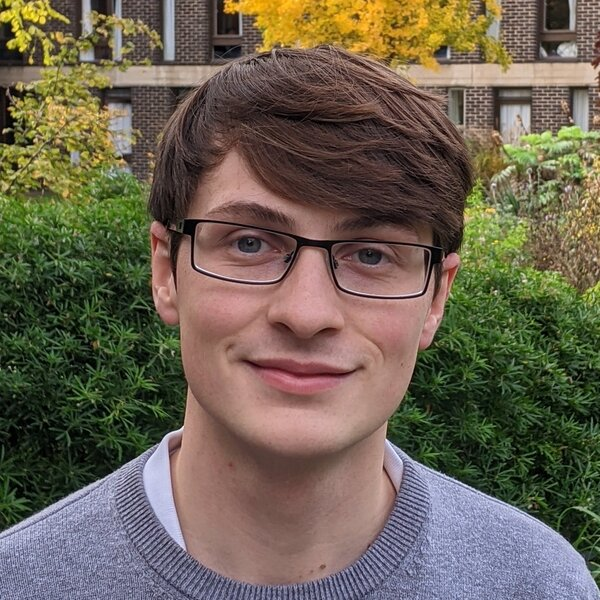
\includegraphics[width=\textwidth]{people/thomas_gessey-jones}
    \end{columns}
\end{frame}

\begin{frame}
    \frametitle{SBI: Simulation-based inference}
    \begin{columns}
        \column{0.5\textwidth}
        \begin{itemize}
            \item What do you do if you don't know \C[2]{$\mathcal{L}(D|\theta)$}?
            \item If you have a simulator/forward model $\theta \rightarrow D$
                defines an \C[2]{\emph{implicit} likelihood~$\mathcal{L}$}.
            \item Simulator generates samples from $\C[2]{\mathcal{L}(\cdot|\theta)}$.
            \item With a \C[1]{prior $\pi(\theta)$} can generate samples from \C[4]{joint distribution}~$\C[4]{\mathcal{J}(\theta,D)}=\C[2]{\mathcal{L}(D|\theta)}\C[1]{\pi(\theta)}$\\\hfill \emph{the ``probability of everything''}.
            \item Task of SBI is take joint~$\C[4]{\mathcal{J}}$ samples and learn \C[0]{posterior $\mathcal{P}(\theta|D)$},  and \C[3]{evidence $\mathcal{Z}(D)$} \\ or even \C[2]{likelihood~$\mathcal{L}(D|\theta)$} or \C[4]{joint~$\mathcal{J}(\theta,D)$}.
            \item Present state of the art achieves this using \emph{machine learning} (neural networks).
        \end{itemize}
        \column{0.5\textwidth}
        \includegraphics<1|handout:0>[page=1, width=\textwidth]{figures/sbi_parameter_estimation.pdf}%
        \includegraphics<2|handout:0>[page=2, width=\textwidth]{figures/sbi_parameter_estimation.pdf}%
        \includegraphics<3|handout:0>[page=3, width=\textwidth]{figures/sbi_parameter_estimation.pdf}%
        \includegraphics<4|handout:0>[page=4, width=\textwidth]{figures/sbi_parameter_estimation.pdf}%
        \includegraphics<5|handout:0>[page=5, width=\textwidth]{figures/sbi_parameter_estimation.pdf}%
        \includegraphics<6|handout:0>[page=6, width=\textwidth]{figures/sbi_parameter_estimation.pdf}%
        \includegraphics<7|handout:0>[page=7, width=\textwidth]{figures/sbi_parameter_estimation.pdf}%
        \includegraphics<8|handout:0>[page=8, width=\textwidth]{figures/sbi_parameter_estimation.pdf}%
        \includegraphics<9|handout:0>[page=9, width=\textwidth]{figures/sbi_parameter_estimation.pdf}%
        \includegraphics<10|handout:0>[page=10, width=\textwidth]{figures/sbi_parameter_estimation.pdf}%
        \includegraphics<11|handout:0>[page=11, width=\textwidth]{figures/sbi_parameter_estimation.pdf}%
        \includegraphics<12|handout:0>[page=12, width=\textwidth]{figures/sbi_parameter_estimation.pdf}%
        \includegraphics<13|handout:0>[page=13, width=\textwidth]{figures/sbi_parameter_estimation.pdf}%
        \includegraphics<14|handout:0>[page=14, width=\textwidth]{figures/sbi_parameter_estimation.pdf}%
        \includegraphics<15|handout:0>[page=15, width=\textwidth]{figures/sbi_parameter_estimation.pdf}%
        \includegraphics<16|handout:0>[page=16, width=\textwidth]{figures/sbi_parameter_estimation.pdf}%
        \includegraphics<17|handout:0>[page=17, width=\textwidth]{figures/sbi_parameter_estimation.pdf}%
        \includegraphics<18|handout:0>[page=18, width=\textwidth]{figures/sbi_parameter_estimation.pdf}%
        \includegraphics<19|handout:0>[page=19, width=\textwidth]{figures/sbi_parameter_estimation.pdf}%
        \includegraphics<20|handout:0>[page=20, width=\textwidth]{figures/sbi_parameter_estimation.pdf}%
        \includegraphics<21>[page=21, width=\textwidth]{figures/sbi_parameter_estimation.pdf}%
    \end{columns}
\end{frame}

\begin{frame}
    \frametitle{Why \textit{linear} SBI?}
    If neural networks are all that, why should we consider the regressive step of going back to linear versions of this problem?

    \begin{itemize}
        \item It is pedagogically helpful 
            \begin{itemize}
                \item separates general principles of SBI from the details of neural networks
                \item (particularly for ML skeptics)
            \end{itemize}
        \item It is practically useful
            \begin{itemize}
                \item for producing expressive examples with known ground truths. 
            \end{itemize}
        \item It is pragmatically useful
            \begin{itemize}
                \item competitive with neural approaches in terms of accuracy,
                \item faster and more interpretable. 
            \end{itemize}
    \end{itemize}
\end{frame}

\begin{frame}
    \frametitle{Linear Simulation Based Inference}
    \framesubtitle{Mathematical setup}
    \begin{columns}[t]
        \column{0.5\textwidth}
        \begin{itemize}
            \item Linear generative model $(m,M,C)$
                \[ 
                    \only<1>{D = m + M \theta \pm \sqrt{C}}%
                    \only<2>{D \sim \mathcal{N}(m + M \theta, C)}%D \sim 
                    %\only<3>{p = \mathcal{N}(D|m + M \theta, C)}
                \]%
                where:
                \begin{description}
                    \item[$\theta$]: $n$ dimensional parameters
                    \item[$D$]: $d$ dimensional data
                    \item[$M$]: $d\times n$ transfer matrix
                    \item[$m$]: $d$-dimensional shift
                    \item[$C$]:  $d\times d$ data covariance
                \end{description}
        \end{itemize}
        
        \pause
        \column{0.5\textwidth}
        \begin{itemize}
            \item $k$ Simulations 
                \[
                    S=\{ (\theta_i,D_i): i=1,\ldots,k\}
                \]
            \item Define simulation statistics\footnotemark:

                \begin{description}
                    \item[$\bar\theta$] $= \tfrac{1}{k}\sum_k \theta_i$
                    \item[$\bar D$] $= \tfrac{1}{k}\sum_k D_i$
                    \item[$\Theta$] $=\tfrac{1}{k-1}\sum_i (\theta_i-\bar\theta)(\theta_i-\bar\theta)'$
                    \item[$\Delta$] $=\tfrac{1}{k-1}\sum_i (D_i-\bar D)(D_i-\bar D)'$
                    \item[$\Psi$] $=\tfrac{1}{k-1}\sum_i (D_i-\bar D)(\theta_i-\bar \theta)'$
                \end{description}
        \end{itemize}
    \end{columns}
    \footnotetext[1]{N.B. using matrix variate notation where primes denote transposes $M' = M^T$}
\end{frame}

\begin{frame}
    \frametitle{Linear Simulation Based Inference: gory mathematical details}
    \begin{columns}
        \column{0.7\textwidth}
        \begin{itemize}
            \item We now wish to infer the parameters of the linear model $(m,M,C)$ from simulations $S$ (which define $\bar\theta,\bar D, \Theta, \Delta, \Psi$)
            \item The likelihood for this problem is:
                \[P(\{D_i\}|\{\theta_i\}|m, M, C) = \prod_i \mathcal{N}(D_i|m+M\theta_i,C)\]
            \item It can be shown the \C[0]{posterior $\mathcal{P}$} is\ldots
                \onslide<3>{
                \begin{align*}
                    m&|M,C,S \sim \mathcal{N}(\tfrac{k}{k+1}(\bar D - M \bar \theta), \tfrac{C}{k+1}), \\
                    M&|C,S \sim \mathcal{MN}(\Psi \Theta^{-1}_*, \tfrac{C}{k-1}, \Theta^{-1}_*), \\
                    C&|S\sim \mathcal{W}^{-1}_\nu(C_0 + (k-1)(\Delta-\Psi \Theta^{-1} \Psi')),
                \end{align*}%
                where $\Theta_* = \tfrac{1}{k-1}\Theta_0 + \Theta$, $\nu=\nu_0+k$, and $C_0$ define conjugate \C[2]{prior $\pi$} on $m,M,C$
            }
        \end{itemize}

        
        \column{0.3\textwidth}
        \includegraphics<2->[width=\textwidth]{figures/matrix_variate_distributions.jpg}
    \end{columns}
\end{frame}

\begin{frame}
    \frametitle{Sequential LSBI}
\end{frame}


\begin{frame}
    \frametitle{Example of this on our toy model}
    \begin{columns}
        \column{0.5\textwidth}
        
        \column{0.5\textwidth}
        \includegraphics<1|handout:0>[width=\textwidth, page=1]{figures/lsbi_plot.pdf}%
        \includegraphics<2|handout:0>[width=\textwidth, page=2]{figures/lsbi_plot.pdf}%
        \includegraphics<3|handout:0>[width=\textwidth, page=3]{figures/lsbi_plot.pdf}%
        \includegraphics<4|handout:0>[width=\textwidth, page=4]{figures/lsbi_plot.pdf}%
        \includegraphics<5|handout:0>[width=\textwidth, page=5]{figures/lsbi_plot.pdf}%
        \includegraphics<6|handout:0>[width=\textwidth, page=6]{figures/lsbi_plot.pdf}%
        \includegraphics<7|handout:0>[width=\textwidth, page=7]{figures/lsbi_plot.pdf}%
        \includegraphics<8|handout:0>[width=\textwidth, page=8]{figures/lsbi_plot.pdf}%
        \includegraphics<9|handout:0>[width=\textwidth, page=9]{figures/lsbi_plot.pdf}%
        \includegraphics<10|handout:0>[width=\textwidth, page=10]{figures/lsbi_plot.pdf}%
        \includegraphics<11|handout:0>[width=\textwidth, page=11]{figures/lsbi_plot.pdf}%
        \includegraphics<12|handout:0>[width=\textwidth, page=12]{figures/lsbi_plot.pdf}%
        \includegraphics<13|handout:0>[width=\textwidth, page=13]{figures/lsbi_plot.pdf}%
        \includegraphics<14|handout:0>[width=\textwidth, page=14]{figures/lsbi_plot.pdf}%
        \includegraphics<15|handout:0>[width=\textwidth, page=15]{figures/lsbi_plot.pdf}%
        \includegraphics<16|handout:0>[width=\textwidth, page=16]{figures/lsbi_plot.pdf}%
    \end{columns}
\end{frame}

\begin{frame}
    \frametitle{Example of this on the CMB}
\end{frame}

\begin{frame}
    \frametitle{\texttt{lsbi}: linear simulation based inference}
    \framesubtitle{Code details}
    \begin{itemize}
        \item \texttt{lsbi} is a pip-installable python package
        \item it extends \texttt{scipy.stats.multivariate\_normal}
            \begin{itemize}
                \item vectorised distributions with (broadcastable) arrays of \texttt{mean} and \texttt{cov}
                \item \texttt{.marginalise(...)} and \texttt{.condition(...)} methods
                \item Plotting functionality
            \end{itemize}
        \item Implements \texttt{LinearModel} class with \texttt{.prior()}, \texttt{.likelihood(theta)}, \texttt{.posterior(D)} \& \texttt{.evidence()} methods which return distributions
        \item Also implement \texttt{MixtureModel}
        \item Under active develpoment
            \begin{itemize}
                \item Open source
                \item Continuous integration
            \end{itemize}
        \item \tthref{github.com/handley-lab/lsbi}
    \end{itemize}

\end{frame}

\begin{frame}
    \frametitle{Where next?}
    \begin{itemize}
        \item Paper being written up 
            \begin{itemize}
                \item soft deadline for Nicolas' MPhil start in October
                \item hard deadline for PhD applications
            \end{itemize}
        \item Include realistic CMB simulation effects (foregrounds)
        \item Extend to more examples (BAO, SNe)
        \item How does LSBI contribute to the question of compression
        \item If the posterior is the answer, what is the question?
    \end{itemize}
\end{frame}

\begin{frame}
    \frametitle{Conclusions}
    \framesubtitle{\tthref{github.com/handley-lab}}
    \tikz[overlay,remember picture]
    \node[anchor=north east] (A) at ($(current page.north east)+(0,0)$) {
        
\includegraphics[width=0.10\textheight]{people/adam_ormondroyd.jpg}%
        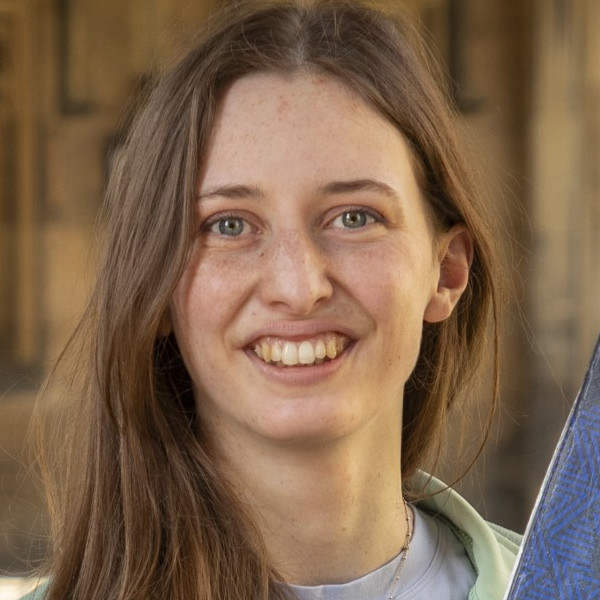
\includegraphics[width=0.10\textheight]{people/charlotte_priestley.jpg}%
        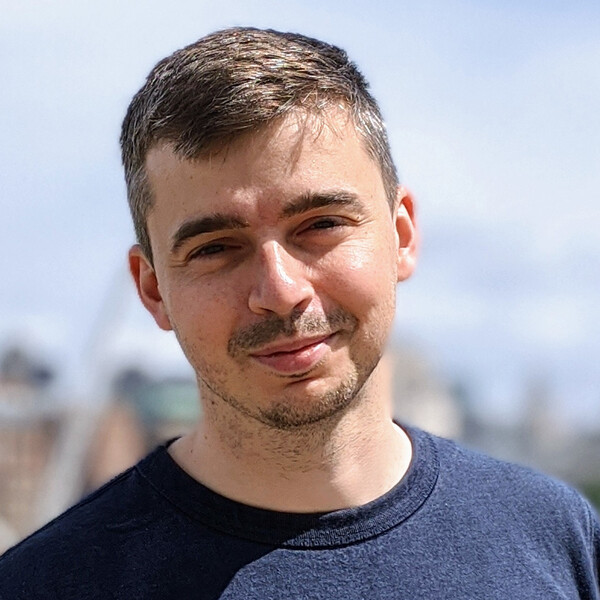
\includegraphics[width=0.10\textheight]{people/david_yallup.jpg}%
        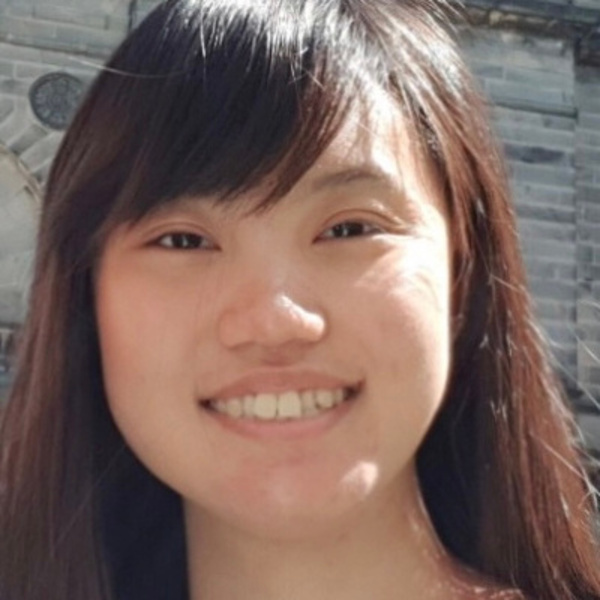
\includegraphics[width=0.10\textheight]{people/dily_ong.jpg}%
        
\includegraphics[width=0.10\textheight]{people/george_carter.jpg}%
        
\includegraphics[width=0.10\textheight]{people/harry_bevins.jpg}%
        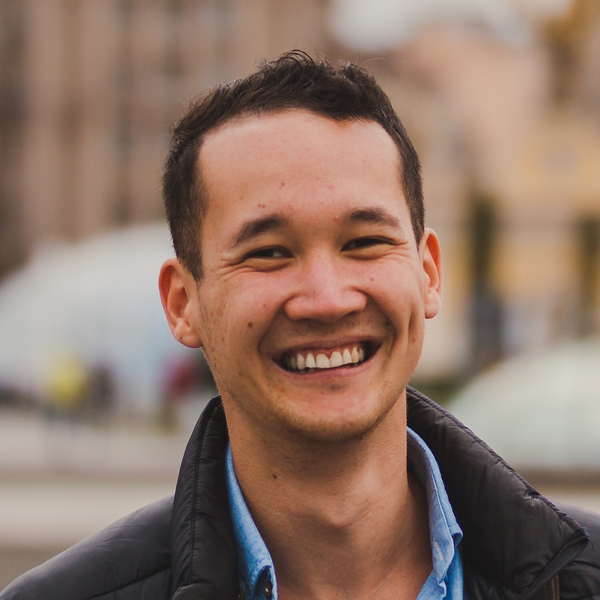
\includegraphics[width=0.10\textheight]{people/kilian_scheutwinkel.jpg}%
        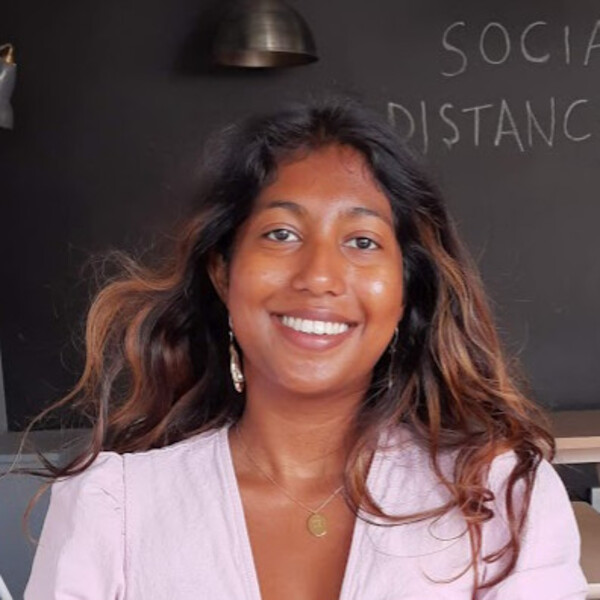
\includegraphics[width=0.10\textheight]{people/metha_prathaban.jpg}%
        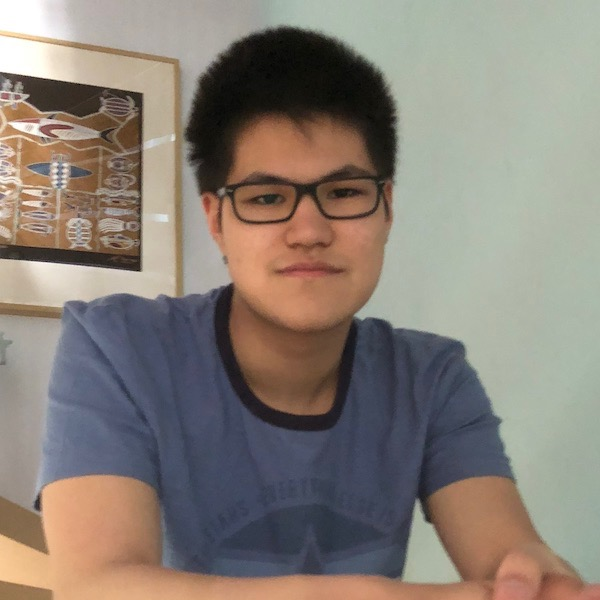
\includegraphics[width=0.10\textheight]{people/namu_kroupa.jpg}%
        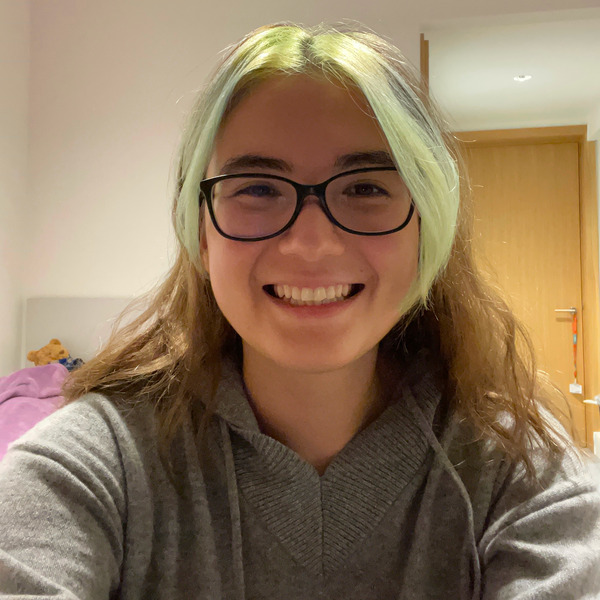
\includegraphics[width=0.10\textheight]{people/sinah_legner.jpg}%
        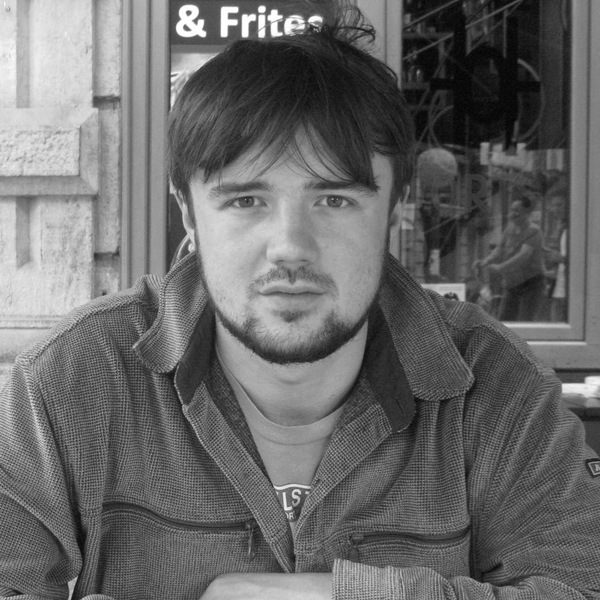
\includegraphics[width=0.10\textheight]{people/sam_leeney.jpg}%
        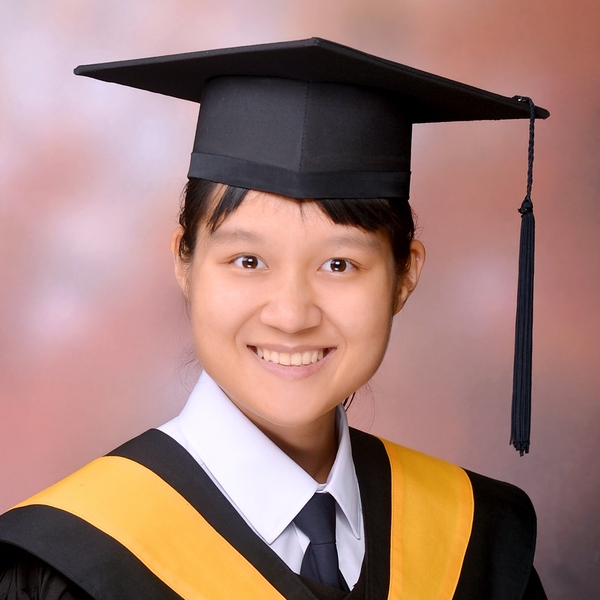
\includegraphics[width=0.10\textheight]{people/wei-ning_deng.jpg}%
        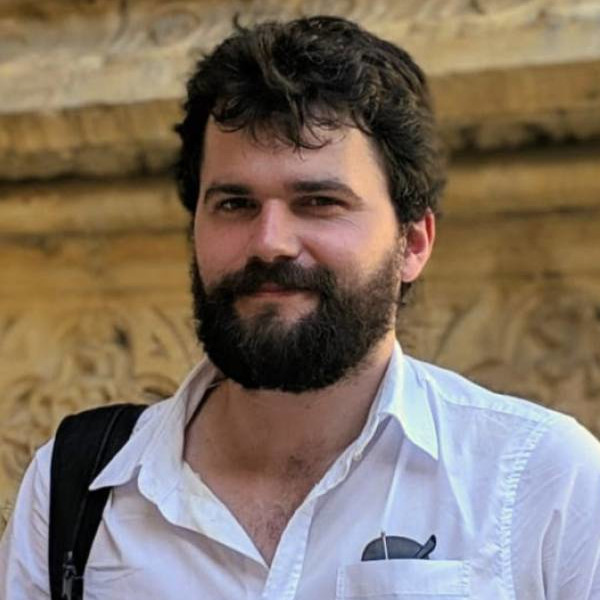
\includegraphics[width=0.10\textheight]{people/will_handley.jpg}%
    };
    \begin{itemize}
        \item 
    \end{itemize}
\end{frame}

\end{document}
